\documentclass[12pt]{article}
\usepackage{epsfig,wrapfig,url,palatino,color,graphicx}
\usepackage{caption}
\usepackage{subcaption}
\graphicspath{{images/}}

\pagestyle{plain}
\renewcommand{\baselinestretch}{1.}

\setlength{\topmargin}{0in}
\setlength{\evensidemargin}{0in}
\setlength{\oddsidemargin}{0in}
\setlength{\headheight}{0in}
\setlength{\headsep}{0in}
\setlength{\footskip}{0.2in}
\setlength{\textheight}{9in}
\setlength{\textwidth}{6.5in}

\renewcommand{\topfraction}{0.99}
\renewcommand{\bottomfraction}{0.99}
\renewcommand{\textfraction}{0.01}
\renewcommand{\floatpagefraction}{0.01}
\renewcommand{\dbltopfraction}{0.99}
\renewcommand{\dblfloatpagefraction}{0.01}

\begin{document}

\noindent
{\bf Title of Proposal:} Evaluation of the usability of a web based 
sketching interface for the iterative design of architectural daylighting \\
{\bf Researcher:}   Max Espinoza\\
{\bf Address:}  MRC 311\\
{\bf Phone:} 518 276 3274\\ 
{\bf Research Advisor (for students):}  Barbara Cutler \\
{\bf Department:}  Computer Science \\
{\bf Is this proposal related to a sponsored project?}  Yes \\
{\bf If yes,  please indicate:}  \\
Existing Award: (Fund \# A12016), NSF, \\
Immersive Architectural Daylighting Design Experience \\

\noindent
All investigators, including faculty supervisors, on this project must
complete the self-study course on protection of human research
subjects. \\
{\bf Certification:  I/We have completed the course:} \\
Max Espinoza (CS PhD Student) 11/09/15 \\ 
Barbara M Cutler
\begin{itemize}
          \item Social and Behavioral Responsible Conduct of Research Course (7/1/2014)
          \item Social/Behavioral Research Course (7/1/2014)
\end{itemize}

\paragraph{Objective:}

Daylighting plays an important role in architecture, its creative and effective use offers occupants aesthetics visuals, increases in productivity, and energy savings. 
In order to realize the benefits of daylight, architects must consider daylighting during the early stages of architecture.
The schematic design phase is an early stage in architecture where architects brainstorm how a space will look and feel. 
Moreover, architects will generally brainstorm on paper through rough architectural sketches and hand drawn floor plans.
Architects will go through many iterations and variations of an idea before committing on a design to show a client.
Additionally, designing a space to effectively use natural lighting is non-trivial  due to its dynamic nature. 
Current software available for daylighting analysis requires time-intensive 3D modeling, which does not capture the spirit of the schematic design phase.
With this in mind, we present a novel online architectural sketching interface for simulations that is easily accessible to non-experts providing them with the tools to perform daylighting analysis during the schematic design phase of an architectural space.
We call this online architectural sketching interface for simulation the Web Interface for the Virtual Heliodon.
For the purpose of evaluating our tool and improving our online architectural sketching interface, we ask participants to both design architectural spaces and perform daylighting simulations.

% Old Objective
% Our goal in this study is to evaluate the effectiveness and usability of 
% our web based sketching interface for the creation of closed architectural 
% geometries and daylighting analysis.

\paragraph{Methods:}
%
Participants in our study will begin by visiting a site hosting the Web Interface for the Virtual Heliodon. 
Afterwards, participants will then register with a username and password of their choosing.
During registration, we will provide a brief explanation about participants' inclusion into our user study.
At the same time, we will also provide an option for participants to opt-out of the user study and still use the Web Interface for the Virtual Heliodon. 
The opt-out option will be clearly displayed when participants are registering. 
Similarly, we will not use any content created by participants who have opted out of the study.
See figure~\ref{fig:registration} on page~\pageref{fig:registration} for a screenshot of the sign-in and registration page. \\

After a successful login, participants will then be taken the main page of the Web Interface for the Virtual Heliodon.
From this point on the application is visually split into two portions. 
On the left-hand side are the tools to make 2D sketches of architectural spaces, convert 2D sketches into 3D models, and view daylighting simulation results. 
On the right-hand side, we provide a feedback panel with questions that participants can answer at any point of the study. 
We do not require that participants answer any feedback questions to continue use of the Web Interface of the Virtual Heliodon. 
Likewise, participants can choose to answer some questions but leave others blank.
Also, participants can stop at any point in time and continue by logging back into our site with their username and password pair.
Ultimately, we designed this user study to be accessible, straightforward, and optional for all our participants. \\

The list of feedback questions we present to our participants is attached at the end of this document. 
Additionally, we include screenshots of the Web Interface for the Virtual Heliodon.

\paragraph{Effects on Subjects:} See Benefits to Participants and Minimization of Possible Risk.

\paragraph{Benefits to Participants:}
%
Participants will gain first-hand experience with a new online architectural sketching environment for the generation of 3D models, in addition to an understanding of the iterative design process of creating architectural spaces. 
Participants will also gain a better understanding of architectural daylighting and the difficulties of designing well-lit space.
Participants will run daylighting simulations and view results through our Web Interface for the Virtual Heliodon to learn more about the lighting of their virtually created space at any given date and time.
On the whole, participants voluntarily providing general feedback helps us, the investigators, evaluate the effectiveness of our 2D architectural sketching interface and our choice in visualizations.

\paragraph{Minimization of Possible Risks:}   
% 
There is no risk of physical harm in our Web Interface for the Virtual Heliodon.
The only tool required to participate in this study is a computer with a modern web browser.
As a result, we have also considered the issue of computer security. 
To protect participants' created content we have a login system that requires a unique username and password pair.
We will also hash participants' password using the SHA-1 hashing algorithm so that nowhere on the system will passwords be stored in plain text.
Likewise, the machine hosting our site will be using an up to date Apache server and hypertext transfer protocol secure (HTTPS) for maximal security. 
The machine we use to host the Web Interface for the Virtual Heliodon is both password protected and situated in a locked office.
This machine is only accessible to the investigators of this study.
To summarize, participants are not required to download anything on their computers to participate in this study, nor will they be required to make security exceptions on firewalls or anti-virus protection software.
Again the Web Interface for the Virtual Heliodon is only dependent on participants having both a computer and web browser ( i.e. Firefox or Google Chrome )\\

We follow standard web security practices on account of the two kinds of digital information participants provide.
Participants will provide and create designs files in the form of 2D architectural sketches and feedback in the form of plain text responses.\\

% Design files
Notably, our application creates design files, a unique encoding of 2D architectural sketches, as participants  use our application.
Participants are encouraged to load previously created 2D architectural sketches and make revisions for daylighting improvements.
As a result, we create and save these design files for both the purpose of the user study and the revision feature. 
We use a PostgreSQL database serviced by the Computer Science Department to store participants' created content. 
Please note that only the investigators have direct access to this database. Furthermore, we store but not use content created by participants who opted out of the study. 
For all participants' convenience, we store all design files to support the revision feature. \\

% Explanation about copyrights
We will be collecting user created content. 
Users retain copyright of designs created in our Web Interface for the Virtual Heliodon.  
Upon registration we, the investigators, will request the right to use both designs and feedback to test our software and as examples in publications.
Users can opt-out of both software-testing research and publication of their designs and feedback.
Lastly, note that all the feedback questions in our survey are optional, including those questions which may be answered with personally identifiable information. 
Namely, we are interested in RPI students to participate in recreating dormitories on our Web Interface for the Virtual Heliodon.
We ask for participants to recreate campus dormitories so that we can evaluate participant's accuracy against blueprints provided by the university.
We also ask questions pertaining to a participants' experience in an architectural space, in order to measure participants' confidence in the recreation of that space.
Some participants may answer vaguely while other participants may answer in great detail with personally identified information.
As a result, we have taken all standard web security measures described above to protect participants' feedback information.

\paragraph{Likelihood of  Harm:}   None

\paragraph{Alternate Method Not Using Human Subjects:} None

\paragraph{Qualifications of Researcher:}
Barbara Cutler has a PhD in Computer Science from Massachusetts
Institute of Technology.  Max Espinoza is a 3th year PhD student in
Computer Science at Rensselaer Polytechnic Institute studying computer
graphics.

\paragraph{Recruiting of Subjects:}
We will ask for anonymous online volunteers to use our site to participate in this user study. 
We will also advertise our site to student volunteers (18 years or older) via posters, campus-related social media, and direct contact with students attending related courses. 
We will obtain permission from course instructors to advertise for the participation of their students, however participation in the study will be voluntary and will not impact their course grade. 
The faculty advisor for the study (Barbara Cutler) will not recruit students in her courses to participate.  
We are particularly interested in participants with experience in 3D modeling, architectural daylighting, general architecture, and visual arts.
We are looking for users with formal education and experience in the above fields to provide us valuable feedback to improve the Web Interface for the Virtual Heliodon's usability and functionality. 
Albeit experience in the above fields is not required for participation in the user study.\\

\noindent Lastly, this study will last for the duration of a year (starting from launch date planned Janurary 25, 2016).
Because this is an online study we plan on reaching a significant number of participants, specifically we aim for 100 participants.

\paragraph{Confidentiality:} 
Participants will register themselves with a username of their choice when logging into the Web Interface for the Virtual Heliodon for the first time. 
We do not require participants use any personally identified usernames and password pairs such as those provided by the RPI (RSC IDs). 
We work under the assumption that participants follow standard practices for the creation and management of their login credential's.
Moreover, participants may optionally provide an email address that will solely be used for follow up questions regarding specific architectural designs.
The emails of the users who did or did not participate in the study will be confidential and will not be released to their instructors. 
These emails will be stored on the machine hosting the Web Interface for the Virtual Heliodon.. 
As mentioned previously, this machine is both password protected and situated in a locked office.
Furthermore, this machine is only accessible to the investigators of this study.
Overall, nowhere in our application will participants be asked for their real name. 

%%%%%%%%%%%%%%%%%%%%%%%%%%%%%%%%%%%%%%%%%%%%%%%%%%%%%%%%%%%%%
%%%%%%%%%%%%%%%%%%%%%%%%%%%%%%%%%%%%%%%%%%%%%%%%%%%%%%%%%%%%%
%%%%%%%%%%%%%%%%%%%%%%%%%%%%%%%%%%%%%%%%%%%%%%%%%%%%%%%%%%%%%

\newpage
\paragraph{Splash-screen Screenshots:}
When participants visit our Web Interface for the Virtual Heliodon they will be directed to a splash-screen page. 
This splash-screen provides users some information about our research and participation in our user study. This screen does not contain details about the user study however. That is information is located on the registration page.Also we simplified the name of our tool from Web Interface for the Virtual Heliodon to the acronym OASIS (Online Architectural Sketching Interface for Simulations).\\

\noindent The transcript of the text:\\

\textbf{What is OASIS?}
OASIS is an online architectural sketching interface for simulations. 
We offer users an easy-to-use interface that allows novices to sketch architectural spaces such as bedrooms, living rooms, and offices spaces. 
Architectural spaces designed in our interface can then be used as input for daylighting simulations. 
This allows non-experts to perform daylighting analysis on their architectural designs.\\

\textbf{Why use OASIS?}
Personal example explaining the picture. 
Have you ever had trouble using your computer, tablet, or TV because of glare coming from the sun outside? 
Glare is one of many issues caused by poor daylighting design and can be fixed through daylighting analysis. 
However, daylighting analysis can be tricky for novices because of the sun's dynamic nature. 
Professional architects rely on small physical models and software to preform daylighting analysis— 
both of which are not available to novice users trying to figure out where to best place their TV or Computer. 
OASIS can be used for the daylighting analysis of existing and imagined architectural spaces. 
It will help you gain a better understanding of how daylighting effects interior spaces and gain an appreciation of the challenges in daylighting analysis.\\

\textbf{Improvement Through User Feedback}
OASIS is a new research tool developed and supported by graduate students at Rensselaer Polytechnic Institute. 
Our goal is to gain insight on daylighting design and improve OASIS through user feedback.
By using our application you can participate and submit feedback to us, the developers and researchers, to help us improve our tool. 
Participants will be given the chance to sketch their architectural spaces in our tool and run daylighting simulations on those spaces. 
Our application is free to use and can be used without participating in our user study. 
Participation is voluntary and may be terminated by you at any point without penalty. 
We will collecting your feedback and architectural designs, no other information will be collected.

\begin{figure}[h]
  \begin{subfigure}{.5\textwidth}
    \centering
    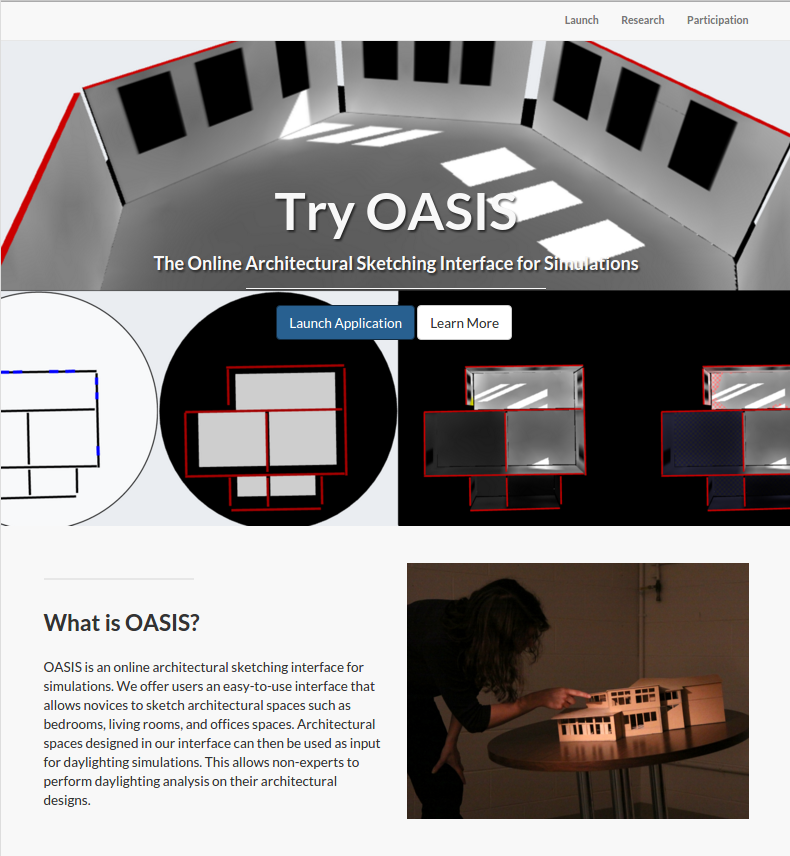
\includegraphics[scale=0.3]{preview}
  \end{subfigure}%
  \begin{subfigure}{.5\textwidth}
    \centering
    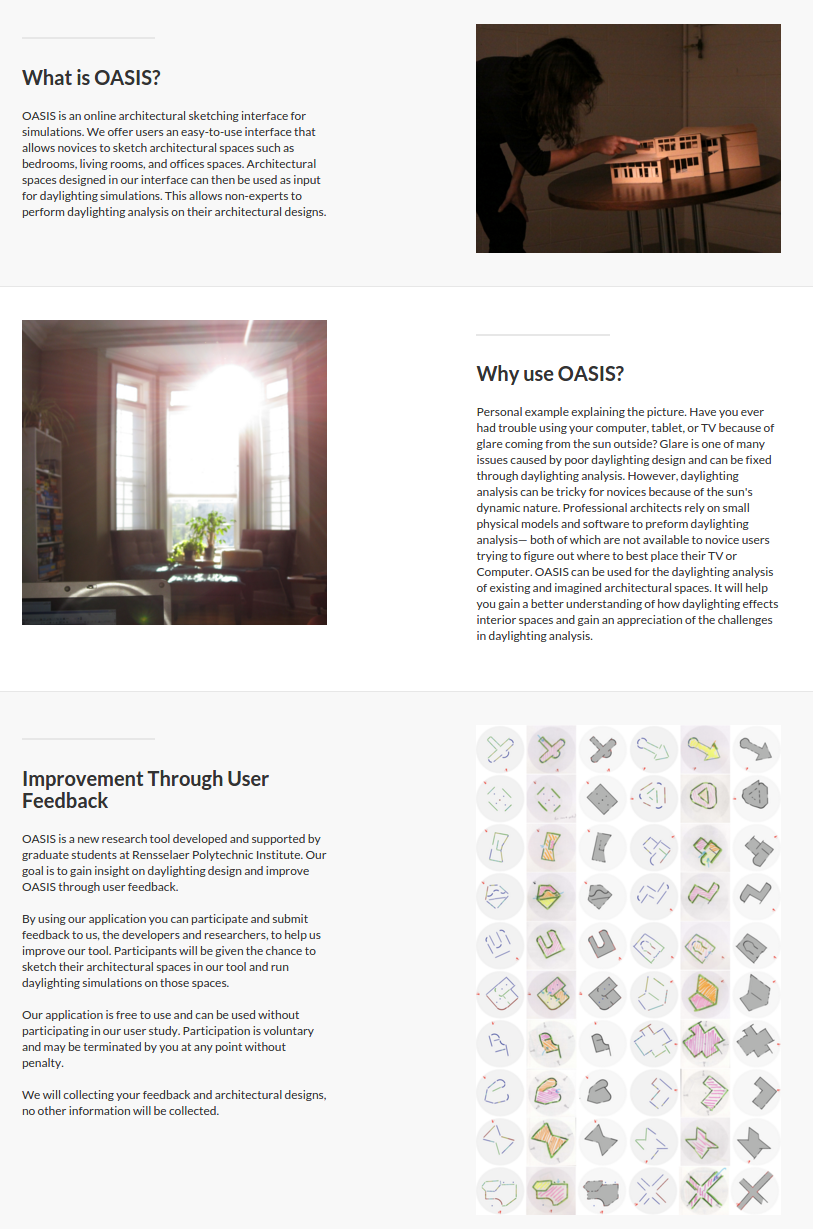
\includegraphics[scale=0.3]{big_img}
  \end{subfigure}

\caption{On the left is what users will see upon first visiting our site (our splash screen). It lets user scroll down to see more information.  On the right is the additional information we provide (transcript above).}  
\label{fig:splash}
\end{figure}
\newpage

%%%%%%%%%%%%%%%%%%%%%%%%%%%%%%%%%%%%%%%%%%%%%%%%%%%%%%%%%%%%%
%%%%%%%%%%%%%%%%%%%%%%%%%%%%%%%%%%%%%%%%%%%%%%%%%%%%%%%%%%%%%
%%%%%%%%%%%%%%%%%%%%%%%%%%%%%%%%%%%%%%%%%%%%%%%%%%%%%%%%%%%%%

\paragraph{Registration and Login Screenshots:}
When participants visit our Web Interface for the Virtual Heliodon they are directed to a registration page. 
However, participants whom previously registered can directly sign into our application. Moreover, during registration there is a brief prompt explaining what information we are recording and an option to opt out of this study.  All other user input beyond this point is optional.\\

\noindent Transcript of text:\\
This application is a research project for architectural modeling and daylighting simulation. Your feedback is important to help us improve this tool. \\
Participation is voluntary. Construction of a model can take anywhere from 5-10 minutes, depending on the complexity and depth of analysis. Your models and written feedback will be collected for use in future publications and to aid in the improvement of our tool. There is no remuneration is offered for participation in this study. \\
Followed by the contact information of the lead investigators and IRB chair.

\begin{figure}[h]
  \begin{subfigure}{.5\textwidth}
    \centering
    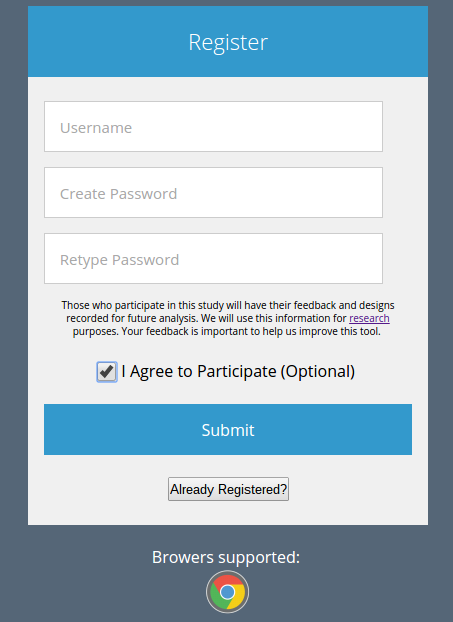
\includegraphics[scale=0.4]{ss_reg}
  \end{subfigure}%
  \begin{subfigure}{.5\textwidth}
    \centering
    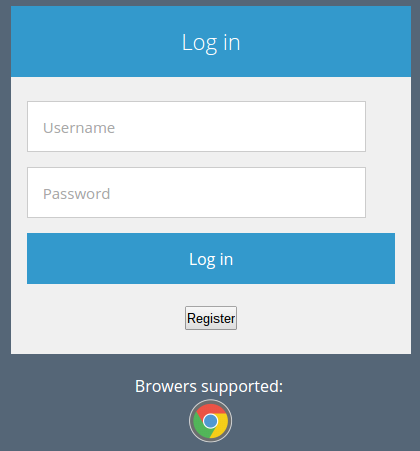
\includegraphics[scale=0.4]{ss_sign}
  \end{subfigure}
\caption{Left) This is the registration page for new participants. Notice the brief statement regarding participation in our user study. Right) Participants will first encounter this sign-in prompt when visiting our site.}  

\label{fig:registration}
\end{figure}

\newpage
\paragraph{Sample User Specific Questions:}
These are sample questions we ask each participant when first logging into the Web Interface for the Virtual Heliodon.
All of these questions are optional, yet we explicitly label some questions optional to remind participants that they are not required to answer. 
We provide screenshots of where these questions are presented in our interface below.

\begin{figure}[h]
\centering
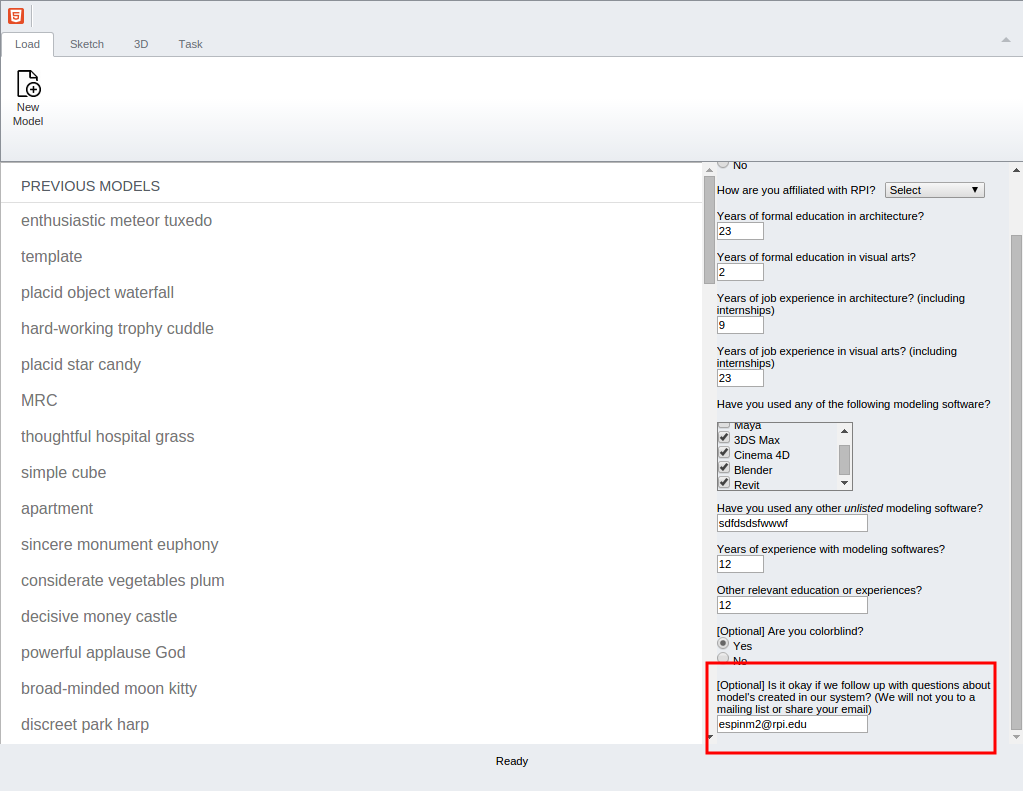
\includegraphics[scale=0.4]{updated_email}
\caption{This is the main page of our Web Interface for the Virtual Heliodon. Notice that questions participants are encouraged to answer are located on the right hand side of the interface. We purposefully placed feedback questions here to avoid being obstructive. Also note the of the page we placed a red block around. We put explicitly state that email's provided will protected. Also that emails will not be shared or put on a mailing list. }
\label{fig:sfig1}
\end{figure}

\begin{enumerate}  
        \item Are you affiliated with Rensselaer Polytechnic Institute? 
        \item How are you affiliated with Rensselaer Polytechnic Institute?
        \item Years of formal education in Architecture?
        \item Years of formal education in Visual Arts?
        \item Years of job experience in architecture? (including internships) 
        \item Years of job experience in Visual Arts? (including internships)
        \item Have you used any of the following modeling software?
        \begin{enumerate}  
          \item SketchUp
          \item AutoCAD
          \item Rhino
          \item Maya
          \item 3DS Max
          \item Cinema 4D
          \item Blender
          \item Revit
          \item Other
        \end{enumerate}
        \item Years of experience with modeling software?
        \item Other relevant education / experience?
        \item Are you colorblind?
        \item Is it okay if we follow up with additional questions about specific models you created in our system?
          \begin{enumerate}
            \item If so, please enter your email address
          \end{enumerate}

    \item What did you find fun or interesting in this sketching environment?
    \item What additional features should be added to system to allow greater flexibility in design?
    \item Describe some designs that you were not able to create due  to system limitations?
    \item Was there anything you did not like about working in this sketching environment?
    \item Where there any UI elements that were hard to use or confusing at first?

    \item Describe your overall impression of the software for determining the interior vs exterior space in your designs?
    \item For the cases when the system’s interpretation of the interior/exterior of your design was incorrect where was the system wrong? 
    \item Did you understand the results of the simulation, was there anything confusing or unclear?
    \item Did the system allow you to create and test daylighting performance with respect to over or under illumination?

      \end{enumerate}

\newpage

\paragraph{Design Specific Sample Questions:}
These are sample questions we will ask per architectural  2D sketch.
Upon the creation of a design these questions will be available for participants to answer.
Again, all of these questions are optional and we remind users that these questions are optional by labeling them as optional. Screenshots of where these questions are presented in our website are provided below.

\begin{figure}[h]
  \begin{subfigure}{.5\textwidth}
    \centering
    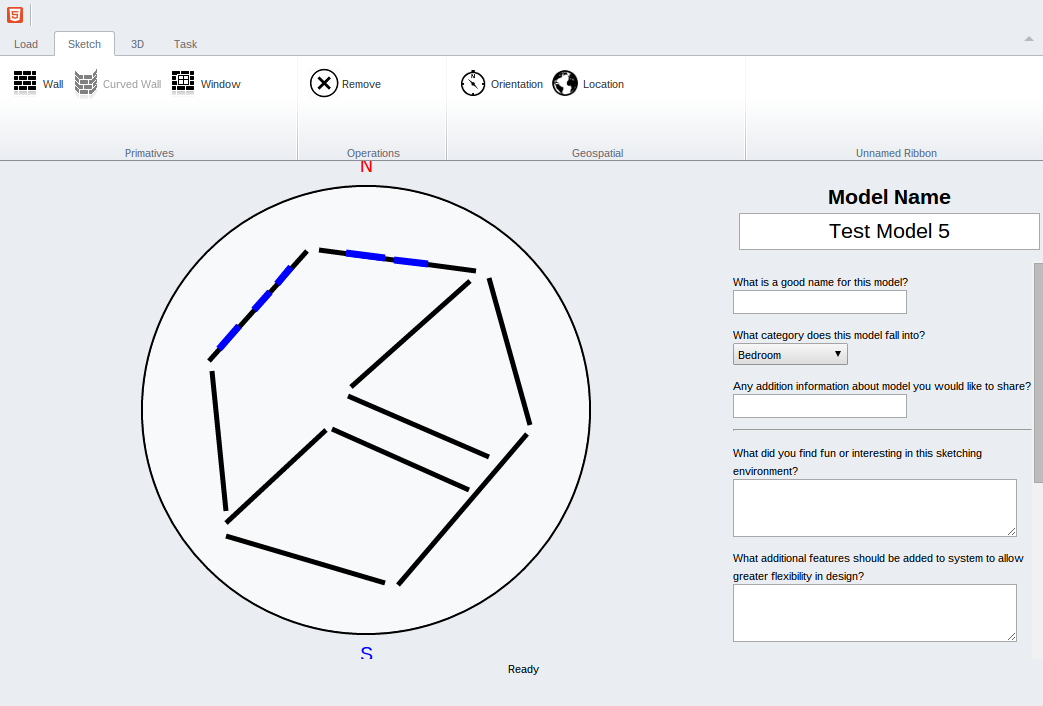
\includegraphics[scale=0.2]{ss_sketch}
    %\caption{Users will create simple designs here by dragging lines across the screen. These designs in addition to feed back are saved for future analysis.}
    %\label{fig:sfig1}
  \end{subfigure}%
  \begin{subfigure}{.5\textwidth}
    \centering
    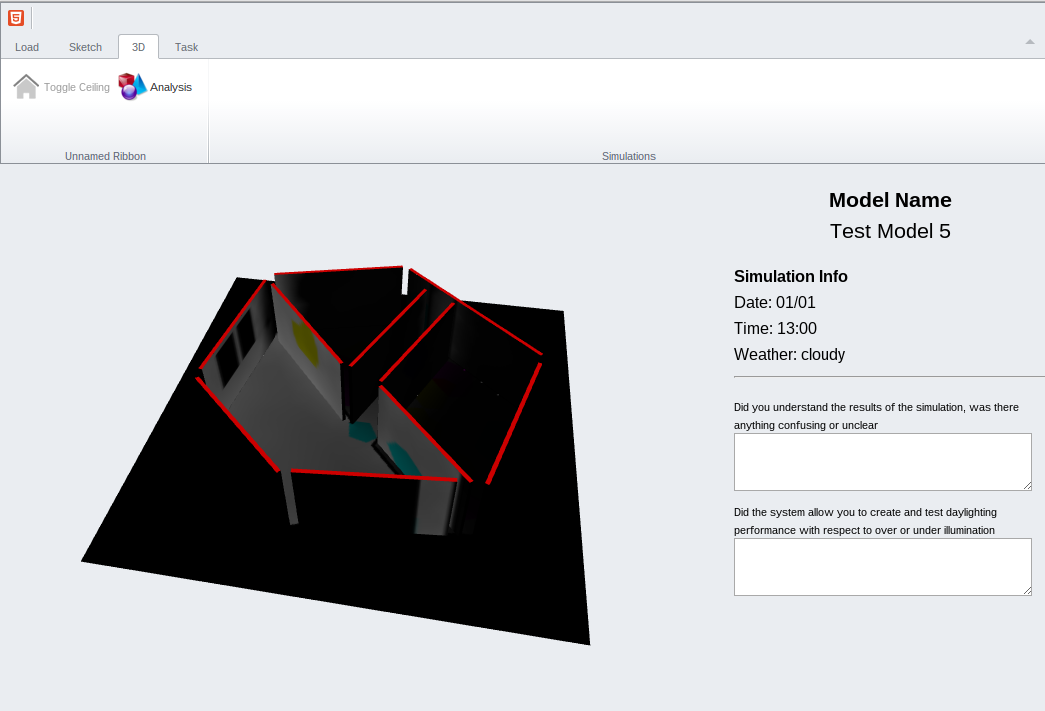
\includegraphics[scale=0.2]{ss_render}
    %\caption{Users visualize the 3D rendering of their designs here. }
    %\label{fig:sfig2}
  \end{subfigure}
\caption{Left) Above is a screenshot the sketching interface where participants create 2D architectural sketches. The designs of participants, that have not opted out, are saved for inclusion into our user study. Moreover, we save these designs with intension of analysing the 2D architectural sketches that our algorithm could not convert into 3D models. This analysis will help us, the investigators, in improving our algorithm for the Web Interface for the Virtual Heliodon.
Right) Participants can also view 3D daylighting simulation results from their 2D architectural sketches. Notice how throughout the application the feedback we are collecting is non-intrusive and located on the right hand side. }
%\label{fig:fig}
\end{figure}

      \begin{enumerate}
        \item What category does this model fall into?
        \begin{enumerate}
          \item Dorm
          \item Bedroom
          \item Living room 
          \item Apartment / House
          \item Classroom
          \item Office
          \item Lobby
          \item Other
        \end{enumerate}
        % If it is an rpi dorm 
      \item What dorm is this a model of? (Optional)
      \begin{enumerate}
        \item BARH (Burdett Avenue Residence Hall)
        \item Barton Hall
        \item Beman Lane Undergraduate RAHP Apartments
        \item Blitman Residence Commons
        \item Bray Hall
        \item Bryckwyck Floor Plans
        \item Cary Hall
        \item Colonie Apartments
        \item Commons
        \item Crockett Hall
        \item Davison Hall
        \item E-Complex
        \item Hall Hall
        \item Nason Hall
        \item North Hall
        \item Nugent Hall
        \item Quadrangle (The Quad)
        \item Sharp Hall
        \item Single RAHP
        \item Stacwyck Apartments
        \item Warren Hall
        \item Other
      \end{enumerate}
    \item What floor number? (Optional)
    \item What room number? (Optional)
    \item When was the last time you visited this space? (Optional)
      \begin{enumerate}
        \item Less than a week ago
        \item Less than a month ago
        \item Less then a year ago
        \item Less than 4 years ago
        \item More than 4 years ago
      \end{enumerate}
    \item How often did you visit this space?
      \begin{enumerate}
        \item Once
        \item Occasionally
        \item Multiple times a week
      \end{enumerate}
    \item How confident are you in modeling this space? (scale of 1 to 5)
    \item Does the 3D generated model match your intentions?
      \begin{enumerate}
        \item Matched my intentions exactly ( no revision required )
        \item Did not match my intentions initially ( revisions were required )
        \item Failed to match my intentions ( even after revision )
      \end{enumerate}
  \end{enumerate}

\newpage 

\end{document}
